% Options for packages loaded elsewhere
% Options for packages loaded elsewhere
\PassOptionsToPackage{unicode}{hyperref}
\PassOptionsToPackage{hyphens}{url}
\PassOptionsToPackage{dvipsnames,svgnames,x11names}{xcolor}
%
\documentclass[
  letterpaper,
  DIV=11,
  numbers=noendperiod]{scrartcl}
\usepackage{xcolor}
\usepackage{amsmath,amssymb}
\setcounter{secnumdepth}{-\maxdimen} % remove section numbering
\usepackage{iftex}
\ifPDFTeX
  \usepackage[T1]{fontenc}
  \usepackage[utf8]{inputenc}
  \usepackage{textcomp} % provide euro and other symbols
\else % if luatex or xetex
  \usepackage{unicode-math} % this also loads fontspec
  \defaultfontfeatures{Scale=MatchLowercase}
  \defaultfontfeatures[\rmfamily]{Ligatures=TeX,Scale=1}
\fi
\usepackage{lmodern}
\ifPDFTeX\else
  % xetex/luatex font selection
\fi
% Use upquote if available, for straight quotes in verbatim environments
\IfFileExists{upquote.sty}{\usepackage{upquote}}{}
\IfFileExists{microtype.sty}{% use microtype if available
  \usepackage[]{microtype}
  \UseMicrotypeSet[protrusion]{basicmath} % disable protrusion for tt fonts
}{}
\makeatletter
\@ifundefined{KOMAClassName}{% if non-KOMA class
  \IfFileExists{parskip.sty}{%
    \usepackage{parskip}
  }{% else
    \setlength{\parindent}{0pt}
    \setlength{\parskip}{6pt plus 2pt minus 1pt}}
}{% if KOMA class
  \KOMAoptions{parskip=half}}
\makeatother
% Make \paragraph and \subparagraph free-standing
\makeatletter
\ifx\paragraph\undefined\else
  \let\oldparagraph\paragraph
  \renewcommand{\paragraph}{
    \@ifstar
      \xxxParagraphStar
      \xxxParagraphNoStar
  }
  \newcommand{\xxxParagraphStar}[1]{\oldparagraph*{#1}\mbox{}}
  \newcommand{\xxxParagraphNoStar}[1]{\oldparagraph{#1}\mbox{}}
\fi
\ifx\subparagraph\undefined\else
  \let\oldsubparagraph\subparagraph
  \renewcommand{\subparagraph}{
    \@ifstar
      \xxxSubParagraphStar
      \xxxSubParagraphNoStar
  }
  \newcommand{\xxxSubParagraphStar}[1]{\oldsubparagraph*{#1}\mbox{}}
  \newcommand{\xxxSubParagraphNoStar}[1]{\oldsubparagraph{#1}\mbox{}}
\fi
\makeatother

\usepackage{color}
\usepackage{fancyvrb}
\newcommand{\VerbBar}{|}
\newcommand{\VERB}{\Verb[commandchars=\\\{\}]}
\DefineVerbatimEnvironment{Highlighting}{Verbatim}{commandchars=\\\{\}}
% Add ',fontsize=\small' for more characters per line
\usepackage{framed}
\definecolor{shadecolor}{RGB}{241,243,245}
\newenvironment{Shaded}{\begin{snugshade}}{\end{snugshade}}
\newcommand{\AlertTok}[1]{\textcolor[rgb]{0.68,0.00,0.00}{#1}}
\newcommand{\AnnotationTok}[1]{\textcolor[rgb]{0.37,0.37,0.37}{#1}}
\newcommand{\AttributeTok}[1]{\textcolor[rgb]{0.40,0.45,0.13}{#1}}
\newcommand{\BaseNTok}[1]{\textcolor[rgb]{0.68,0.00,0.00}{#1}}
\newcommand{\BuiltInTok}[1]{\textcolor[rgb]{0.00,0.23,0.31}{#1}}
\newcommand{\CharTok}[1]{\textcolor[rgb]{0.13,0.47,0.30}{#1}}
\newcommand{\CommentTok}[1]{\textcolor[rgb]{0.37,0.37,0.37}{#1}}
\newcommand{\CommentVarTok}[1]{\textcolor[rgb]{0.37,0.37,0.37}{\textit{#1}}}
\newcommand{\ConstantTok}[1]{\textcolor[rgb]{0.56,0.35,0.01}{#1}}
\newcommand{\ControlFlowTok}[1]{\textcolor[rgb]{0.00,0.23,0.31}{\textbf{#1}}}
\newcommand{\DataTypeTok}[1]{\textcolor[rgb]{0.68,0.00,0.00}{#1}}
\newcommand{\DecValTok}[1]{\textcolor[rgb]{0.68,0.00,0.00}{#1}}
\newcommand{\DocumentationTok}[1]{\textcolor[rgb]{0.37,0.37,0.37}{\textit{#1}}}
\newcommand{\ErrorTok}[1]{\textcolor[rgb]{0.68,0.00,0.00}{#1}}
\newcommand{\ExtensionTok}[1]{\textcolor[rgb]{0.00,0.23,0.31}{#1}}
\newcommand{\FloatTok}[1]{\textcolor[rgb]{0.68,0.00,0.00}{#1}}
\newcommand{\FunctionTok}[1]{\textcolor[rgb]{0.28,0.35,0.67}{#1}}
\newcommand{\ImportTok}[1]{\textcolor[rgb]{0.00,0.46,0.62}{#1}}
\newcommand{\InformationTok}[1]{\textcolor[rgb]{0.37,0.37,0.37}{#1}}
\newcommand{\KeywordTok}[1]{\textcolor[rgb]{0.00,0.23,0.31}{\textbf{#1}}}
\newcommand{\NormalTok}[1]{\textcolor[rgb]{0.00,0.23,0.31}{#1}}
\newcommand{\OperatorTok}[1]{\textcolor[rgb]{0.37,0.37,0.37}{#1}}
\newcommand{\OtherTok}[1]{\textcolor[rgb]{0.00,0.23,0.31}{#1}}
\newcommand{\PreprocessorTok}[1]{\textcolor[rgb]{0.68,0.00,0.00}{#1}}
\newcommand{\RegionMarkerTok}[1]{\textcolor[rgb]{0.00,0.23,0.31}{#1}}
\newcommand{\SpecialCharTok}[1]{\textcolor[rgb]{0.37,0.37,0.37}{#1}}
\newcommand{\SpecialStringTok}[1]{\textcolor[rgb]{0.13,0.47,0.30}{#1}}
\newcommand{\StringTok}[1]{\textcolor[rgb]{0.13,0.47,0.30}{#1}}
\newcommand{\VariableTok}[1]{\textcolor[rgb]{0.07,0.07,0.07}{#1}}
\newcommand{\VerbatimStringTok}[1]{\textcolor[rgb]{0.13,0.47,0.30}{#1}}
\newcommand{\WarningTok}[1]{\textcolor[rgb]{0.37,0.37,0.37}{\textit{#1}}}

\usepackage{longtable,booktabs,array}
\newcounter{none} % for unnumbered tables
\usepackage{calc} % for calculating minipage widths
% Correct order of tables after \paragraph or \subparagraph
\usepackage{etoolbox}
\makeatletter
\patchcmd\longtable{\par}{\if@noskipsec\mbox{}\fi\par}{}{}
\makeatother
% Allow footnotes in longtable head/foot
\IfFileExists{footnotehyper.sty}{\usepackage{footnotehyper}}{\usepackage{footnote}}
\makesavenoteenv{longtable}
\usepackage{graphicx}
\makeatletter
\newsavebox\pandoc@box
\newcommand*\pandocbounded[1]{% scales image to fit in text height/width
  \sbox\pandoc@box{#1}%
  \Gscale@div\@tempa{\textheight}{\dimexpr\ht\pandoc@box+\dp\pandoc@box\relax}%
  \Gscale@div\@tempb{\linewidth}{\wd\pandoc@box}%
  \ifdim\@tempb\p@<\@tempa\p@\let\@tempa\@tempb\fi% select the smaller of both
  \ifdim\@tempa\p@<\p@\scalebox{\@tempa}{\usebox\pandoc@box}%
  \else\usebox{\pandoc@box}%
  \fi%
}
% Set default figure placement to htbp
\def\fps@figure{htbp}
\makeatother


% definitions for citeproc citations
\NewDocumentCommand\citeproctext{}{}
\NewDocumentCommand\citeproc{mm}{%
  \begingroup\def\citeproctext{#2}\cite{#1}\endgroup}
\makeatletter
 % allow citations to break across lines
 \let\@cite@ofmt\@firstofone
 % avoid brackets around text for \cite:
 \def\@biblabel#1{}
 \def\@cite#1#2{{#1\if@tempswa , #2\fi}}
\makeatother
\newlength{\cslhangindent}
\setlength{\cslhangindent}{1.5em}
\newlength{\csllabelwidth}
\setlength{\csllabelwidth}{3em}
\newenvironment{CSLReferences}[2] % #1 hanging-indent, #2 entry-spacing
 {\begin{list}{}{%
  \setlength{\itemindent}{0pt}
  \setlength{\leftmargin}{0pt}
  \setlength{\parsep}{0pt}
  % turn on hanging indent if param 1 is 1
  \ifodd #1
   \setlength{\leftmargin}{\cslhangindent}
   \setlength{\itemindent}{-1\cslhangindent}
  \fi
  % set entry spacing
  \setlength{\itemsep}{#2\baselineskip}}}
 {\end{list}}
\usepackage{calc}
\newcommand{\CSLBlock}[1]{\hfill\break\parbox[t]{\linewidth}{\strut\ignorespaces#1\strut}}
\newcommand{\CSLLeftMargin}[1]{\parbox[t]{\csllabelwidth}{\strut#1\strut}}
\newcommand{\CSLRightInline}[1]{\parbox[t]{\linewidth - \csllabelwidth}{\strut#1\strut}}
\newcommand{\CSLIndent}[1]{\hspace{\cslhangindent}#1}



\setlength{\emergencystretch}{3em} % prevent overfull lines

\providecommand{\tightlist}{%
  \setlength{\itemsep}{0pt}\setlength{\parskip}{0pt}}



 


\KOMAoption{captions}{tableheading}
\makeatletter
\@ifpackageloaded{caption}{}{\usepackage{caption}}
\AtBeginDocument{%
\ifdefined\contentsname
  \renewcommand*\contentsname{Table of contents}
\else
  \newcommand\contentsname{Table of contents}
\fi
\ifdefined\listfigurename
  \renewcommand*\listfigurename{List of Figures}
\else
  \newcommand\listfigurename{List of Figures}
\fi
\ifdefined\listtablename
  \renewcommand*\listtablename{List of Tables}
\else
  \newcommand\listtablename{List of Tables}
\fi
\ifdefined\figurename
  \renewcommand*\figurename{Figure}
\else
  \newcommand\figurename{Figure}
\fi
\ifdefined\tablename
  \renewcommand*\tablename{Table}
\else
  \newcommand\tablename{Table}
\fi
}
\@ifpackageloaded{float}{}{\usepackage{float}}
\floatstyle{ruled}
\@ifundefined{c@chapter}{\newfloat{codelisting}{h}{lop}}{\newfloat{codelisting}{h}{lop}[chapter]}
\floatname{codelisting}{Listing}
\newcommand*\listoflistings{\listof{codelisting}{List of Listings}}
\makeatother
\makeatletter
\makeatother
\makeatletter
\@ifpackageloaded{caption}{}{\usepackage{caption}}
\@ifpackageloaded{subcaption}{}{\usepackage{subcaption}}
\makeatother
\usepackage{bookmark}
\IfFileExists{xurl.sty}{\usepackage{xurl}}{} % add URL line breaks if available
\urlstyle{same}
\hypersetup{
  pdftitle={RChASM: An R Package for Identifying Nonmosaic Whole-chromosome Aneuploidies from Low-coverage Sequence Data},
  colorlinks=true,
  linkcolor={blue},
  filecolor={Maroon},
  citecolor={Blue},
  urlcolor={Blue},
  pdfcreator={LaTeX via pandoc}}


\title{RChASM: An R Package for Identifying Nonmosaic Whole-chromosome
Aneuploidies from Low-coverage Sequence Data}
\author{Adam B. Rohrlach \and Jonathan Tuke \and Kay
Prüfer \and Wolfgang Haak}
\date{2026-11-06}
\begin{document}
\maketitle


\newcommand{\bm}[1]{\boldsymbol{#1}}
\newcommand{\apprsim}{%
  \mathrel{\ooalign{\hss$\sim$\hss\cr
                    \hidewidth\raise0.65ex\hbox{$\cdot$}\hidewidth\cr
                    \hidewidth\lower0.65ex\hbox{$\cdot$}\hidewidth}}%
}

\section{Summary}\label{summary}

A (non-mosaic) chromosomal aneuploidy is defined as the presence of an
abnormal number of chromosomes, deviating from the common 46 (Orr et al.
2015). These aneuploidies represent one of the most common causes of
large-scale genetic abnormality, frequently resulting in spontaneous
miscarriage(Hassold and Hunt 2001). Autosomal aneuploidies specifically
affect chromosomes 1 to 22, occur in approximately one in 800 live
births (Nagaoka et al. 2012), and are termed a monosomy or trisomy when
there is a loss or gain of a copy of a chromosome, respectively (Orr et
al. 2015). All autosomal trisomies, except for trisomies 13 (Patau
syndrome), 18 (Edwards syndrome) or 21 (Down syndrome), lead to
embryonic or fetal loss, however trisomies 13 and 18 remain associated
with high rates of prenatal loss and severely limited postnatal life
expectancy. Sex chromosomal aneuploidies affect only the X and Y
chromosomes, with XXY (Klinefelter syndrome), XYY (Jacobs syndrome), XXX
(Triple X syndrome) and X0 (Turner syndrome) being the most common
karyotypes, are more common, occurring in approximately one in 450 live
births ({Samango-Sprouse et al.} 2013). The phenotypic traits associated
with sex chromosomal aneuploidies are much milder than those associated
with autosomal aneuploidies, so much so that they often go unnoticed and
hence undiagnosed, but can still lead to developmental issues and
increased disease risk factors (Skuse et al. 2018, hong2014cognitive).

Here we present the R-package \texttt{RChASM} (the
\textbf{R}-implementation of the \textbf{Ch}romosomal
\textbf{A}neuploidy \textbf{S}creening \textbf{M}ethodology framework),
which implements the concepts introduced by ChASM (Rohrlach et al.
2026): an R-package for identifying chromosomal aneuploidies in
low-coverage ancient DNA data sets. \texttt{RChASM} utilises a
Dirichlet-multinomial distribution, trained on a reference set of
``similar'' DNA sequence data, to model the proportion of reads mapping
to each chromosome. Due to this reference distribution, \texttt{RChASM}
returns posterior probabilities for the autosomal karyotypes trisomies
13, 18 and 21 (or no autosomal aneuploidy), as well as sex chromosomal
karyotypes XX, XY, XXY, XYY, XXX and X0. \texttt{RChASM} also produces
diagnostic plots and statistics for diagnosing fit to the reference
distribution or whether contamination is driving karyotype assignment.
Our approach allows ancient DNA researchers to confidently assign
autosomal and sex chromosomal karyotypes for data with as few as 60,000
mapped reads, or approximately 0.001X mean coverage.

\section{Statement of need}\label{statement-of-need}

\texttt{RChASM} is an R package for use in ancient DNA studies, and any
studies looking to identify chromosomal aneuploidies from extremely
low-coverage DNA sequence data, such as in the forensic sciences.
\texttt{RChASM} is designed to be a user-friendly software package,
which takes as input read counts mapping to each chromosome, or a text
file defining the paths to a collection of bam files. \texttt{RChASM}
does not rely on pre-calculated values or parameters, and instead trains
a bespoke Dirichlet-multinomial model on the reference data provided,
which need contain only around 30 realisations, allowing \texttt{RChASM}
to be applied to any type of human sequence data.

\section{State of the field}\label{state-of-the-field}

Only one other method currently exists in the literature:
Karyo\(R_{x}R_{y}\) ({Anastasiadou et al.} 2024). Karyo\(R_{x}R_{y}\)
also calculates the proportion of reads mapping to each chromosome,
however, instead of modeling the reads via a reference distribution,
Karyo\(R_{x}R_{y}\) uses pre-calculated thresholds. These thresholds,
which are equivalent to boundary rectangles, are defined for XXY, XYY,
XXX and X0, and for trisomy 21 for the autosomes. Karyo\(R_{x}R_{y}\)
takes as input a bam file and whether the sequence data is the result of
shotgun ({Venter et al.} 2001) or 1240k capture ({Mathieson et al.}
2018) sequencing data.

Due to the fact that Karyo\(R_{x}R_{y}\) uses a model-free approach with
pre-calculated thresholds, there are three critical differences between
it and \texttt{RChASM}. First, Karyo\(R_{x}R_{y}\) can be run on a
single individual without need for a reference set, where
\texttt{RChASM} requires at least 30 observations to be used as
reference data. Second, as a result of this, Karyo\(R_{x}R_{y}\) can
only be applied to shotgun or 1240k sequence data. Third, due to this
model-free approach, Karyo\(R_{x}R_{y}\) produces no posterior
probabilities for karyotype assignment or diagnostic plots to assess
model fit. However, we always encourage researchers to use multiple
methods when analysing low-coverage sequence data, and would suggest
that both methods be applied.

\section{Modeling the proportion of reads mapping to each
chromosome}\label{modeling-the-proportion-of-reads-mapping-to-each-chromosome}

Consider for some individual \(j\), a set of chromosomes \(A\), where
\(|A|=n\), and let \(\mathbf{N}_j=\left(N_{1j},\cdots,N_{nj}\right)\) be
the number of reads mapping to each chromosome, where \(N_j\) is the
total number of reads. Note that we use three chromosomal sets: the
autosomal set \(A_a = \left\{1,\cdots,22 \right\}\), the sex chromosomal
set \(A_s = \left\{A_a,X,Y \right\}\) and the set for calculating
Z-scores \(A_z = A_a\setminus \left\{13,18,21\right\}\).

Define also a vector \(\mathbf{c} = \left[c_i\right]\),
\(i=1,\cdots,n\), to be the expected fold-increase in the number of
reads mapping to chromosome \(i\), compared to an ``average'\,'
individual. For example, if all \(c_i=1\) except \(c_{21}=1.5\), this
would represent a 50\% increase in the reads mapping to chromosome 21,
and hence trisomy 21 (Down syndrome).

Let \(\mathbf{p}^{\mathbf{c}}\) be the probability vector that models
the expected proportion of reads mapping to each chromosome. However,
because DNA preservation, and sequencing protocols create additional
uncertainty, \(\mathbf{N}_j\) cannot be modeled using a simple
multinomial distribution. Instead, we let
\(\mathbf{p}^{\mathbf{c}} \sim Dirichlet\left(\boldsymbol{\alpha}\right)\)
be a conjugate prior, and hence have that the posterior distribution for
\(\boldsymbol{N}_j\) is a Dirichlet-multinomial (DM) distribution of the
form

\[
\boldsymbol{N}_j \sim DM\left(N_j,\boldsymbol{\alpha}\right),
\]

where

\[
\boldsymbol{\alpha} = \left(\alpha_1,\cdots,\alpha_n \right),
\]

and

\[
\alpha_0 = \sum_{i=1}^{n}\alpha_i.
\]

We then perform parameter estimation to find \(\boldsymbol{\alpha}\)
from a quality-filtered reference data set with a sample size of at
least 30 (Rohrlach et al. 2026). We find three \(\boldsymbol{\alpha}\)
vectors, one for the autosomes
(\(\boldsymbol{\alpha}^{\boldsymbol{c}^{1}_{a}}\)), and one each for
genetically-male (\(\boldsymbol{\alpha}^{XY}\)) and genetically-female
(\(\boldsymbol{\alpha}^{XX}\)) individuals. Note that we estimate
\(\boldsymbol{\alpha}^{XX}\) as it allows us to estimate the expected
proportion of reads mapping to the Y chromosome, due to sequencing and
mapping error, when there is no Y chromosome (denoted \(\epsilon^+\)).

From this reference distribution, we can calculate the expected number
of reads mapping to chromosome \(i\), for individual \(j\) as

\[
\mu_{ij} = N_{j}\dfrac{\alpha_i}{\alpha_0},
\] with standard error \[
\sigma_{ij} = \sqrt{N_j\dfrac{\alpha_i}{\alpha_0}\left(1-\dfrac{\alpha_i}{\alpha_0} \right) \left(\dfrac{N_j + \alpha_i}{1 + \alpha_0} \right)}.
\]

For an unobserved karyotype defined by
\(\boldsymbol{c}^* = \left[k_i\right]\), a new mapping probability
vector \(\boldsymbol{\alpha}^{\boldsymbol{c}^*}\) can be constructed by
setting

\[
\boldsymbol{\alpha}^{\boldsymbol{c}^*} = \left[ k_i \alpha_i \right].
\]

We can now calculate the probability of observing the read count
distribution \(\boldsymbol{N}_j\) that we see, given the karyotype
\(\boldsymbol{c}^* \in \boldsymbol{\kappa}\), denoted
\(P\left( \boldsymbol{N}_j \big\vert \boldsymbol{\alpha}, \boldsymbol{c}^* \right)\).

Hence, posterior probabilities can be calculated for each karyotype of
interest of the form

\[
P\left(\boldsymbol{c}^*\big\vert \boldsymbol{N}_j,\boldsymbol{\alpha}\right) = \dfrac{P\left( \boldsymbol{N}_j \big\vert \boldsymbol{\alpha}, \boldsymbol{c}^* \right)P\left(\boldsymbol{c}^* \right)}{\sum_{\kappa_i\in\boldsymbol{\kappa}} P\left( \boldsymbol{N}_j \big\vert \boldsymbol{\alpha}, \boldsymbol{c}^{\kappa_i} \right)},
\]

where \(P\left(\boldsymbol{c}^* \right)\) is the probability of a
karyotype, estimated from modern medical literature.

Finally, for individual \(j\), a Z-score can be calculated comparing the
observed to the expected number of reads mapping to chromosome \(i\) as,

\[
    Z_{ij} = \dfrac{N_{ij}-\mu_{ij}}{\sigma_{ij}},
\]

with an overall goodness-of-fit statistic of the form

\[
    \lambda_{j} = \sum_{i=1}^{n} Z_{ij}^2,
\] where

\[
    \lambda_j %
  \mathrel{\ooalign{\hss$\sim$\hss\cr
                    \hidewidth\raise 0.65ex\hbox{$\cdot$}\hidewidth\cr
                    \hidewidth\lower 0.65ex\hbox{$\cdot$}\hidewidth}}%
\chi^2_{n}.
\]

\section{Example usage}\label{example-usage}

The package \texttt{RChASM} is available under the MIT license from the
Comprehensive R Archive Network (CRAN) at
\href{https://CRAN.R-project.org/package=RChASM}{https://CRAN.R-project.org/package=RChASM}.
The package can be installed and loaded using the following command:

\begin{Shaded}
\begin{Highlighting}[]
\SpecialCharTok{\textgreater{}} \FunctionTok{install.packages}\NormalTok{(}\AttributeTok{pkgs=}\StringTok{"RChASM"}\NormalTok{)}
\end{Highlighting}
\end{Shaded}

To show an example of how one might use \texttt{RChASM} we use the
inbuilt data set \texttt{example\_data}, which can be loaded into R
using the commands:

\begin{Shaded}
\begin{Highlighting}[]
\SpecialCharTok{\textgreater{}} \FunctionTok{library}\NormalTok{(RChASM)}
\SpecialCharTok{\textgreater{}} \FunctionTok{data}\NormalTok{(example\_data)}
\end{Highlighting}
\end{Shaded}

This data is empirical data that has been anonymised, but had known
cases of chromosomal aneuploidies from published studies (Rohrlach et
al. 2026).

\subsection{Pre-processing bam files}\label{pre-processing-bam-files}

\texttt{RChASM} takes as input the number of reads mapping to each of
the chromosomes: 1-22, X and Y. An individual ID must be given for each
observation and, optionally, a ``protocol'' (an identifier stating the
method that was used to generate the data). The protocol is only
important if mixed types of data are given in a single analysis, and
which \texttt{RChASM} will treat as independent analyses with
independent DM distributions, although the results will be combined in
the final step.

The read count data should have as many rows as you have sequence data,
and then 26 columns for the sample ID, the protocol and the read counts
for all 24 chromosomes (25 columns if no protocol is given).

\begin{Shaded}
\begin{Highlighting}[]
\SpecialCharTok{\textgreater{}}\NormalTok{   sample  protocol    chr1  chr2 chr21 chr22 ...     X     Y}
\SpecialCharTok{\textgreater{}}   \ErrorTok{\textless{}}\NormalTok{chr}\SpecialCharTok{\textgreater{}}   \ErrorTok{\textless{}}\NormalTok{chr}\SpecialCharTok{\textgreater{}}      \ErrorTok{\textless{}}\NormalTok{dbl}\SpecialCharTok{\textgreater{}} \ErrorTok{\textless{}}\NormalTok{dbl}\SpecialCharTok{\textgreater{}} \ErrorTok{\textless{}}\NormalTok{dbl}\SpecialCharTok{\textgreater{}} \ErrorTok{\textless{}}\NormalTok{dbl}\SpecialCharTok{\textgreater{}}\NormalTok{ ... }\SpecialCharTok{\textless{}}\NormalTok{dbl}\SpecialCharTok{\textgreater{}} \ErrorTok{\textless{}}\NormalTok{dbl}\SpecialCharTok{\textgreater{}}
\ErrorTok{\textgreater{}} \DecValTok{1}\NormalTok{ Ind\_1\_1 Protocol }\DecValTok{1}  \DecValTok{7471}  \DecValTok{7955}  \DecValTok{1151}  \DecValTok{1209}\NormalTok{ ...  }\DecValTok{4725}     \DecValTok{5}
\SpecialCharTok{\textgreater{}} \DecValTok{2}\NormalTok{ Ind\_1\_2 Protocol }\DecValTok{1}  \DecValTok{4248}  \DecValTok{4206}   \DecValTok{631}   \DecValTok{760}\NormalTok{ ...  }\DecValTok{2382}     \DecValTok{2}
\SpecialCharTok{\textgreater{}} \DecValTok{3}\NormalTok{ Ind\_3\_1 Protocol }\DecValTok{1}  \DecValTok{9839}  \DecValTok{9935}  \DecValTok{1487}  \DecValTok{1779}\NormalTok{ ...  }\DecValTok{2968}   \DecValTok{235}
\SpecialCharTok{\textgreater{}} \DecValTok{4}\NormalTok{ Ind\_4\_1 Protocol }\DecValTok{1} \DecValTok{34248} \DecValTok{35719}  \DecValTok{5193}  \DecValTok{5707}\NormalTok{ ... }\DecValTok{21254}    \DecValTok{12}
\SpecialCharTok{\textgreater{}} \DecValTok{5}\NormalTok{ Ind\_5\_1 Protocol }\DecValTok{1}  \DecValTok{2306}  \DecValTok{2357}   \DecValTok{356}   \DecValTok{397}\NormalTok{ ...  }\DecValTok{1484}     \DecValTok{1}
\SpecialCharTok{\textgreater{}} \DecValTok{6}\NormalTok{ Ind\_6\_1 Protocol }\DecValTok{1} \DecValTok{58317} \DecValTok{59471}  \DecValTok{8866} \DecValTok{10206}\NormalTok{ ... }\DecValTok{17742}  \DecValTok{1576}
\end{Highlighting}
\end{Shaded}

Listing 1: An example of data that RChASM analyses (omitting columns for
chromosomes 3 to 20).

We supply a simple bash script for pre-processing bam files given a text
file with no column name, and where every line is the path to an indexed
bam file. The script can be downloaded through \texttt{RChASM} by using
the following command in the R terminal:

\begin{Shaded}
\begin{Highlighting}[]
\SpecialCharTok{\textgreater{}} \FunctionTok{system.file}\NormalTok{(}\StringTok{"extdata"}\NormalTok{, }\StringTok{"CHASM\_input.sh"}\NormalTok{, }\AttributeTok{package =} \StringTok{"RChASM"}\NormalTok{)}
\end{Highlighting}
\end{Shaded}

\subsection{Running ChASM in R}\label{running-chasm-in-r}

Once your read counts have been read into R as a data frame or tibble, a
full screening and assignment of both autosomal and sex chromosomal
aneuploidies can be performed using the \texttt{runChASM()} function.
The only input parameter without a default is the read count data, but
there are a further six input parameters that can be set to refine your
analysis (see \autoref{tab:runChASM}). However, the default parameters
have been chosen based on simulation studies, ensuring the most
individuals can be analysed while retaining high statistical power
(Rohrlach et al. 2026).

\begin{longtable}[]{@{}
  >{\raggedright\arraybackslash}p{(\linewidth - 4\tabcolsep) * \real{0.3833}}
  >{\raggedright\arraybackslash}p{(\linewidth - 4\tabcolsep) * \real{0.3333}}
  >{\raggedright\arraybackslash}p{(\linewidth - 4\tabcolsep) * \real{0.2833}}@{}}
\caption{Descriptions of parameters with default values for the
\protect\texttt{runChASM()}
function.\label{tab:runChASM}}\tabularnewline
\toprule\noalign{}
\begin{minipage}[b]{\linewidth}\raggedright
\textbf{Parameter}
\end{minipage} & \begin{minipage}[b]{\linewidth}\raggedright
\textbf{Default}
\end{minipage} & \begin{minipage}[b]{\linewidth}\raggedright
\textbf{Description}
\end{minipage} \\
\midrule\noalign{}
\endfirsthead
\toprule\noalign{}
\begin{minipage}[b]{\linewidth}\raggedright
\textbf{Parameter}
\end{minipage} & \begin{minipage}[b]{\linewidth}\raggedright
\textbf{Default}
\end{minipage} & \begin{minipage}[b]{\linewidth}\raggedright
\textbf{Description}
\end{minipage} \\
\midrule\noalign{}
\endhead
\bottomrule\noalign{}
\endlastfoot
minSamplesPerProtocol & 30 & The minimum number of samples \emph{per
protocol}. Cannot be less than 23. \\
min\_reads & \(6\times 10^{4}\) & The minimum number of total mapped
reads for a sample to be used in the Dirichlet-multinomial parameter
estimation \\
max\_reads & \(1\times 10^{9}\) & The maximum number of total reads for
a sample to be used in the Dirichlet-multinomial parameter estimation \\
p\_contamination & 0.01 & The prior probability of a sample containing
both XX and XY reads due to contamination \\
show\_plot & \texttt{TRUE} & A boolean variable for whether to show
(\texttt{TRUE}) or not to show (\texttt{FALSE}) the clustering results
for the sex chromosomal training set \\
printMissingIDs & \texttt{FALSE} & When merging the autosomal and sex
chromosomal analyses, should missing IDs be printed (\texttt{TRUE}) or
returned as a count (\texttt{FALSE}) \\
\end{longtable}

An analysis of the example\_data using default values can be run using
the command:

\begin{Shaded}
\begin{Highlighting}[]
\NormalTok{example\_calls }\OtherTok{\textless{}{-}} \FunctionTok{runChASM}\NormalTok{(}\AttributeTok{rawReadCountsIn =}\NormalTok{ example\_data)}
\end{Highlighting}
\end{Shaded}

This function runs two separate analyses, one each for the sex
chromosomal and the autosomal aneuploidies, that processes the data,
fits the prior distribution, and then calls the karyotypes. These
analyses are then merged into one result, together with the required
Z-scores. However, only the sex chromosomal clustering plot is visible
(see \autoref{tab:runChASM} and \autoref{fig:clustering}). This figure
is important for assessing that two distinct clusters have been found,
and that the XX cluster has a mean Y-rate value close to zero, and a
mean X-rate that is approximately twice that of the XY cluster.

\begin{figure}[H]

{\centering \pandocbounded{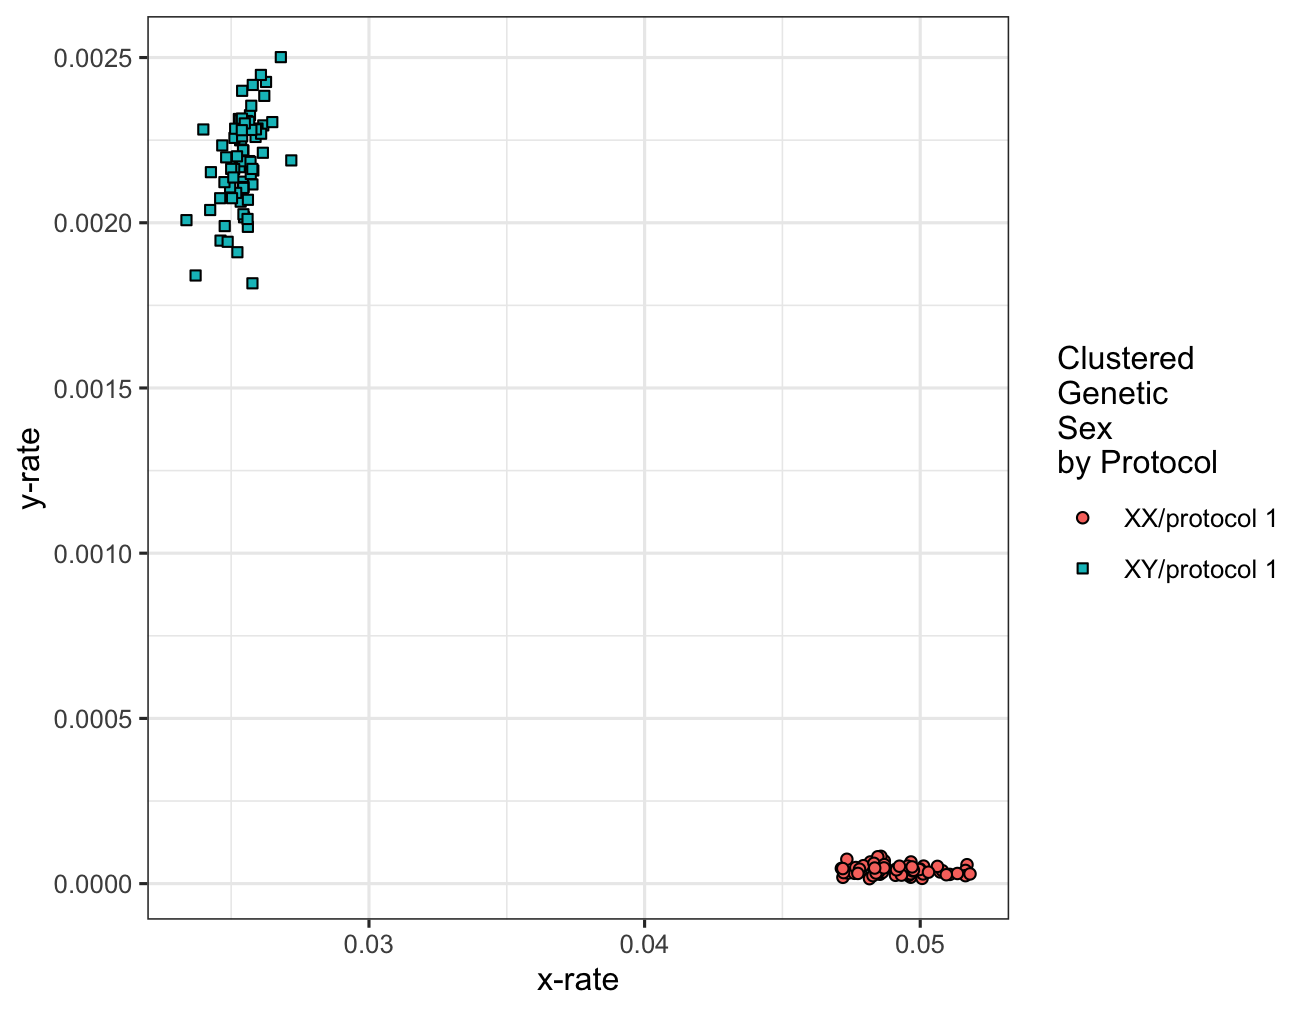
\includegraphics[keepaspectratio]{figs/runChASM_cluster.png}}

}

\caption{The X- and Y-rate values of the samples used for training the
sex chromosomal Dirichlet-multinomial distribution. The samples are
filtered for total read counts, and then clustered into two majority
clusters: XX (red) and XY (blue). It is important that this plot shows
two reasonable clusters, as can be seen in the analysis of the
example\_data.\label{fig:clustering}}

\end{figure}%

The \texttt{runChASM()} function will return a list with the merged
karyotype results (\emph{karyotypes}), the two separate autosomal
(\emph{karyotypes.auto}) and sex chromosomal aneuploidies
(\emph{karyotypes.sca}), the per-protocol parameters of the Dirichlet
distributions for the autosomes (\emph{dirichlet.auto}) and the sex
chromosomes (\emph{dirichlet.sca}), the Z-scores (\emph{z.scores}), as
well as the settings used for the analysis (as described in
\autoref{tab:runChASM}). These results can be examined manually, but we
provide functions for an automated exploration and visualisation of the
analysis or individual results.

\subsection{Interpreting results and diagnostic
plots}\label{interpreting-results-and-diagnostic-plots}

Once the analysis has been successfully completed, interpreting the
results, and assessing goodness-of-fit via summary statistics and
diagnostic plots is critical to reporting the findings.

A summary of all of the results can be printed to screen using the
\texttt{printChASM()} function, which by default prints twenty lines of
output, but can print any number (up to the maximum number of lines) by
setting the \texttt{lines} parameter. For example, the first ten lines
of the full merged analysis of the example\_data can be viewed (up to
the ninth column) using the following command:

\begin{figure}

\centering{

\begin{Shaded}
\begin{Highlighting}[]
\SpecialCharTok{\textgreater{}} \FunctionTok{printChASM}\NormalTok{(}\AttributeTok{inChASM =}\NormalTok{ example\_calls, }\AttributeTok{lines =} \DecValTok{10}\NormalTok{)}
\SpecialCharTok{\textgreater{}}\NormalTok{    sample   protocol   unusual flags autosomal\_call sca\_call C\_call       autosomal\_total sca\_total}
\SpecialCharTok{\textgreater{}}    \ErrorTok{\textless{}}\NormalTok{chr}\SpecialCharTok{\textgreater{}}    \ErrorTok{\textless{}}\NormalTok{chr}\SpecialCharTok{\textgreater{}}      \ErrorTok{\textless{}}\NormalTok{lgl}\SpecialCharTok{\textgreater{}}   \ErrorTok{\textless{}}\NormalTok{int}\SpecialCharTok{\textgreater{}} \ErrorTok{\textless{}}\NormalTok{chr}\SpecialCharTok{\textgreater{}}          \ErrorTok{\textless{}}\NormalTok{chr}\SpecialCharTok{\textgreater{}}    \ErrorTok{\textless{}}\NormalTok{chr}\SpecialCharTok{\textgreater{}}                  \ErrorTok{\textless{}}\NormalTok{dbl}\SpecialCharTok{\textgreater{}}     \ErrorTok{\textless{}}\NormalTok{dbl}\SpecialCharTok{\textgreater{}}
\ErrorTok{\textgreater{}}  \DecValTok{1}\NormalTok{ Ind\_1\_1  protocol }\DecValTok{1} \ConstantTok{TRUE}        \DecValTok{3}\NormalTok{ No Aneuploidy  XX       No Sig XX}\SpecialCharTok{+}\NormalTok{XY           }\DecValTok{89539}     \DecValTok{94269}
\SpecialCharTok{\textgreater{}}  \DecValTok{2}\NormalTok{ Ind\_1\_2  protocol }\DecValTok{1} \ConstantTok{FALSE}       \DecValTok{1}\NormalTok{ No Aneuploidy  XX       No Sig XX}\SpecialCharTok{+}\NormalTok{XY           }\DecValTok{48376}     \DecValTok{50760}
\SpecialCharTok{\textgreater{}}  \DecValTok{3}\NormalTok{ Ind\_3\_1  protocol }\DecValTok{1} \ConstantTok{TRUE}        \DecValTok{2}\NormalTok{ No Aneuploidy  XY       No Sig XX}\SpecialCharTok{+}\NormalTok{XY          }\DecValTok{113335}    \DecValTok{116538}
\SpecialCharTok{\textgreater{}}  \DecValTok{4}\NormalTok{ Ind\_4\_1  protocol }\DecValTok{1} \ConstantTok{FALSE}       \DecValTok{0}\NormalTok{ No Aneuploidy  XX       No Sig XX}\SpecialCharTok{+}\NormalTok{XY          }\DecValTok{406472}    \DecValTok{427738}
\SpecialCharTok{\textgreater{}}  \DecValTok{5}\NormalTok{ Ind\_5\_1  protocol }\DecValTok{1} \ConstantTok{FALSE}       \DecValTok{0}\NormalTok{ No Aneuploidy  XX       No Sig XX}\SpecialCharTok{+}\NormalTok{XY           }\DecValTok{27731}     \DecValTok{29216}
\SpecialCharTok{\textgreater{}}  \DecValTok{6}\NormalTok{ Ind\_6\_1  protocol }\DecValTok{1} \ConstantTok{FALSE}       \DecValTok{0}\NormalTok{ No Aneuploidy  XY       No Sig XX}\SpecialCharTok{+}\NormalTok{XY          }\DecValTok{681256}    \DecValTok{700574}
\SpecialCharTok{\textgreater{}}  \DecValTok{7}\NormalTok{ Ind\_7\_2  protocol }\DecValTok{1} \ConstantTok{FALSE}       \DecValTok{0}\NormalTok{ No Aneuploidy  XY       No Sig XX}\SpecialCharTok{+}\NormalTok{XY          }\DecValTok{130928}    \DecValTok{134684}
\SpecialCharTok{\textgreater{}}  \DecValTok{8}\NormalTok{ Ind\_9\_1  protocol }\DecValTok{1} \ConstantTok{FALSE}       \DecValTok{0}\NormalTok{ No Aneuploidy  XX       No Sig XX}\SpecialCharTok{+}\NormalTok{XY          }\DecValTok{425906}    \DecValTok{448296}
\SpecialCharTok{\textgreater{}}  \DecValTok{9}\NormalTok{ Ind\_15\_1 protocol }\DecValTok{1} \ConstantTok{FALSE}       \DecValTok{1}\NormalTok{ No Aneuploidy  XX       No Sig XX}\SpecialCharTok{+}\NormalTok{XY            }\DecValTok{3364}      \DecValTok{3530}
\SpecialCharTok{\textgreater{}} \DecValTok{10}\NormalTok{ Ind\_17\_1 protocol }\DecValTok{1} \ConstantTok{FALSE}       \DecValTok{1}\NormalTok{ No Aneuploidy  XY       No Sig XX}\SpecialCharTok{+}\NormalTok{XY           }\DecValTok{11699}     \DecValTok{12023}
\end{Highlighting}
\end{Shaded}

}

\caption{\label{fig-printChasmOutput}The result of passing the RChASM
analysis of the example data to the \texttt{printChASM()} function, with
only the first ten lines printed (omitting the last two columns for
visualisation)\label{fig:printChasmOutput}.}

\end{figure}%

This output can be saved as a TSV by passing the full analysis to the
\texttt{saveChASM()} function, and can be sorted by sample name. To save
the sorted analysis of the example\_data, we can use the following
command:

\begin{Shaded}
\begin{Highlighting}[]
\SpecialCharTok{\textgreater{}} \FunctionTok{saveChASM}\NormalTok{(}\AttributeTok{inChASM =}\NormalTok{ example\_calls, }
            \AttributeTok{file =} \StringTok{"\textasciitilde{}/Downloads/example\_analysis.tsv"}\NormalTok{, }
            \AttributeTok{sort\_by\_samplename =} \ConstantTok{TRUE}\NormalTok{)}
\end{Highlighting}
\end{Shaded}

\subsubsection{Uncommon karyotypes - analysis
overview}\label{uncommon-karyotypes---analysis-overview}

A summary of the individuals for which uncommon autosomal (trisomies 13,
18 and 21) and sex chromosomal (XXY, XYY, XXX and X0) aneuploidies were
the karyotypes with highest posterior probabilities can be made with the
\texttt{summary\_calls()} function.

Further filtering for samples and changes to the output columns can be
done with four optional input parameters (see
\autoref{tab:summary_calls}). We again suggest a lower bound on the
number of observed reads of 60,000, but this threshold can be lowered
(reliably to 10,000) for, say, calling genetic sex. Similarly, we
suggest a minimum for the maximum posterior probability of 0.95 in
general, but encourage higher certainty for uncommon karyotypes with a
value of 0.99. It is possible to omit samples that are ``unusual''
(i.e., that have a significant chi-squared goodness-of-fit statistic).
However, as this statistic can be quite sensitive, we encourage users to
inspect this statistic in context with the z-score plot (see panel B in
\autoref{fig:diagnosticT21}).

\begin{longtable}[]{@{}
  >{\raggedright\arraybackslash}p{(\linewidth - 4\tabcolsep) * \real{0.3333}}
  >{\raggedright\arraybackslash}p{(\linewidth - 4\tabcolsep) * \real{0.3958}}
  >{\raggedright\arraybackslash}p{(\linewidth - 4\tabcolsep) * \real{0.2708}}@{}}
\caption{Descriptions of parameters with default values for the
\protect\texttt{summary\_calls()}
function\label{tab:summary_calls}.}\tabularnewline
\toprule\noalign{}
\begin{minipage}[b]{\linewidth}\raggedright
Parameter
\end{minipage} & \begin{minipage}[b]{\linewidth}\raggedright
Default
\end{minipage} & \begin{minipage}[b]{\linewidth}\raggedright
Description
\end{minipage} \\
\midrule\noalign{}
\endfirsthead
\toprule\noalign{}
\begin{minipage}[b]{\linewidth}\raggedright
Parameter
\end{minipage} & \begin{minipage}[b]{\linewidth}\raggedright
Default
\end{minipage} & \begin{minipage}[b]{\linewidth}\raggedright
Description
\end{minipage} \\
\midrule\noalign{}
\endhead
\bottomrule\noalign{}
\endlastfoot
minTotal & \(6\times 10^{4}\) & The minimum number of reads for a sample
to be included in the summary output \\
minPosterior & \(0.95\) & The minimum posterior probability for a result
to be included in the summary output \\
ignoreUnusual & \texttt{FALSE} & A boolean variable indicating if
samples with a significant goodness-of-fit statistic \(\lambda_j\)
should be displayed (\texttt{FALSE}) or omitted (\texttt{TRUE}) in the
summary output \\
printProtocol & \texttt{FALSE} & A boolean variable indicating if the
protocol needs to be included (\texttt{TRUE}) or not (\texttt{FALSE}) in
the summary output \\
\end{longtable}

To generate this summary for the analysis of the example\_data, and
quickly identify the three individuals with uncommon karyotypes, we use
the following command:

\begin{Shaded}
\begin{Highlighting}[]
\SpecialCharTok{\textgreater{}} \FunctionTok{summary\_calls}\NormalTok{(}\AttributeTok{inChASM =}\NormalTok{ example\_calls)}
\SpecialCharTok{\textgreater{}}\NormalTok{   sample    unusual flags autosomal\_call sca\_call C\_call       autosomal\_total sca\_total}
\SpecialCharTok{\textgreater{}}   \ErrorTok{\textless{}}\NormalTok{chr}\SpecialCharTok{\textgreater{}}     \ErrorTok{\textless{}}\NormalTok{lgl}\SpecialCharTok{\textgreater{}}   \ErrorTok{\textless{}}\NormalTok{int}\SpecialCharTok{\textgreater{}} \ErrorTok{\textless{}}\NormalTok{chr}\SpecialCharTok{\textgreater{}}          \ErrorTok{\textless{}}\NormalTok{chr}\SpecialCharTok{\textgreater{}}    \ErrorTok{\textless{}}\NormalTok{chr}\SpecialCharTok{\textgreater{}}        \ErrorTok{\textless{}}\NormalTok{dbl}\SpecialCharTok{\textgreater{}}           \ErrorTok{\textless{}}\NormalTok{dbl}\SpecialCharTok{\textgreater{}}
\ErrorTok{\textgreater{}} \DecValTok{1}\NormalTok{ Ind\_71\_1  }\ConstantTok{TRUE}    \DecValTok{4}\NormalTok{     No Aneuploidy  XXX      No Sig XX}\SpecialCharTok{+}\NormalTok{XY }\DecValTok{70688}           \DecValTok{76444}
\SpecialCharTok{\textgreater{}} \DecValTok{2}\NormalTok{ Ind\_185\_1 }\ConstantTok{FALSE}   \DecValTok{1}\NormalTok{     No Aneuploidy  XXX      No Sig XX}\SpecialCharTok{+}\NormalTok{XY }\DecValTok{209933}          \DecValTok{225713}
\SpecialCharTok{\textgreater{}} \DecValTok{3}\NormalTok{ Ind\_255\_1 }\ConstantTok{FALSE}   \DecValTok{0}\NormalTok{     Trisomy }\DecValTok{21}\NormalTok{     XX       No Sig XX}\SpecialCharTok{+}\NormalTok{XY }\DecValTok{254544}          \DecValTok{268132}
\end{Highlighting}
\end{Shaded}

Listing 2: An overall summary of the uncommon karyotypes found by
passing the RChASM analysis of the example data to the
\texttt{summary\_calls()} function. Note that, although these columns
are omitted for readability, all three individuals have a posterior
probability assigned with their autosomal and sex chromosomal karyotypes
of one (to machine precision)\label{fig:summary_callsOutput}.

We now investigate these two cases of XXX syndrome (Ind\_71\_1 and
Ind\_185\_1) and one case of trisomy 21 (Ind\_255\_1) looking at the
summary statistics and diagnostic plots for goodness-of-fit.

\subsubsection{Producing diagnostic plots and goodness-of-fit summary
statistics}\label{producing-diagnostic-plots-and-goodness-of-fit-summary-statistics}

If an uncommon karyotype is detected in an individual, goodness-of-fit
should be considered. First, it should be decided if the sample even
matches the reference distribution well enough to be able to use the
posterior probability. To do this we consider two things: the
significance of the goodness-of-fit statistic \(\lambda_j\), and the
number of significant Z-scores for the autosomes (denoted \texttt{flags}
in the \texttt{RChASM} output summary). The chromosome associated with
significant Z-scores can be identified via the diagnostic plot (panel B,
\autoref{fig:diagnosticT21}) as the points lying outside of the dashed
lines, which represent two standard deviations from the expected value.

Note that with 22 chromosomes, we expect at least one significant
Z-score by chance. We also find through simulations that \(\lambda_j\)
can be quite sensitive (Rohrlach et al. 2026) to even small
perturbations to the read count distribution. Hence, we suggest
considering a sample poorly fit if \(\lambda_j\) is significant
(`\texttt{unusual\textquotesingle{}\textquotesingle{}\ is}TRUE`) and if
flags \(\geq3\).

Second, it must be considered if the loss or gain in reads to the target
chromosome makes sense in context. For example, if we observe a trisomy
21, then 50\% more reads should be mapping to chromosome 21 than for the
average sample. The diagnostic displays this information for sex
chromosomal karyotypes via a scatter plot of the X- and Y-rate of the
target individual(s), with a random sample of reference individuals for
comparison (panel A, \autoref{fig:diagnosticT21}). This can also be seen
in the fold-increase panel which shows the percentage change in observed
read counts compared to the expected value for an XY individual (panel
C, \autoref{fig:diagnosticT21}).

The analysis summary indicates that Ind\_255\_1 may have the autosomal
karyotype of trisomy 21. From \autoref{tab:summary_calls} we see that
this individual is genetically female (XX) and has a non-significant
\(\lambda_j\) value, indicating that the remaining read counts are
behaving as expected.

To generate a diagnostic plot (see \autoref{fig:diagnosticT21}) for just
this individual, the following command is used:

\begin{Shaded}
\begin{Highlighting}[]
\SpecialCharTok{\textgreater{}} \FunctionTok{plot\_diagnostic}\NormalTok{(}\AttributeTok{IDs =} \StringTok{\textquotesingle{}Ind\_255\_1\textquotesingle{}}\NormalTok{,}
                  \AttributeTok{inChASM =}\NormalTok{ example\_calls, }
                  \AttributeTok{addLabels =} \ConstantTok{TRUE}\NormalTok{)}
\end{Highlighting}
\end{Shaded}

For any given individual (or several individuals), a diagnostic plot can
be produced using the \texttt{plot\_diagnostic()} function. This
function requires the name of the individual of interest, and in this
example, the panels can be interpreted in the following way:

A. Ind\_255\_1 falls within the variation of other XX individuals (and
the sex chromosomal karyotype appears to be XX in this case). B. Except
for chromosome 21, all read counts are within reasonable variability
(\(\pm2\) standard deviations), confirming that the call of trisomy 21
is not due to artefacts in the sequencing sample preservation. C. There
are approximately 48\% more reads mapping to chromosome 21 than
expected, consistent with an extra copy of chromosome 21 being present
(trisomy 21). We also see that we have twice as many copies of the X
chromosome and basically no copies of the Y chromosome (compared to XY),
consistent with XX. We also see (from the legend) that Ind\_255\_1 was
produced using ``protocol 1'' and had 268,132 mapped reads.

\begin{figure}[H]

{\centering \pandocbounded{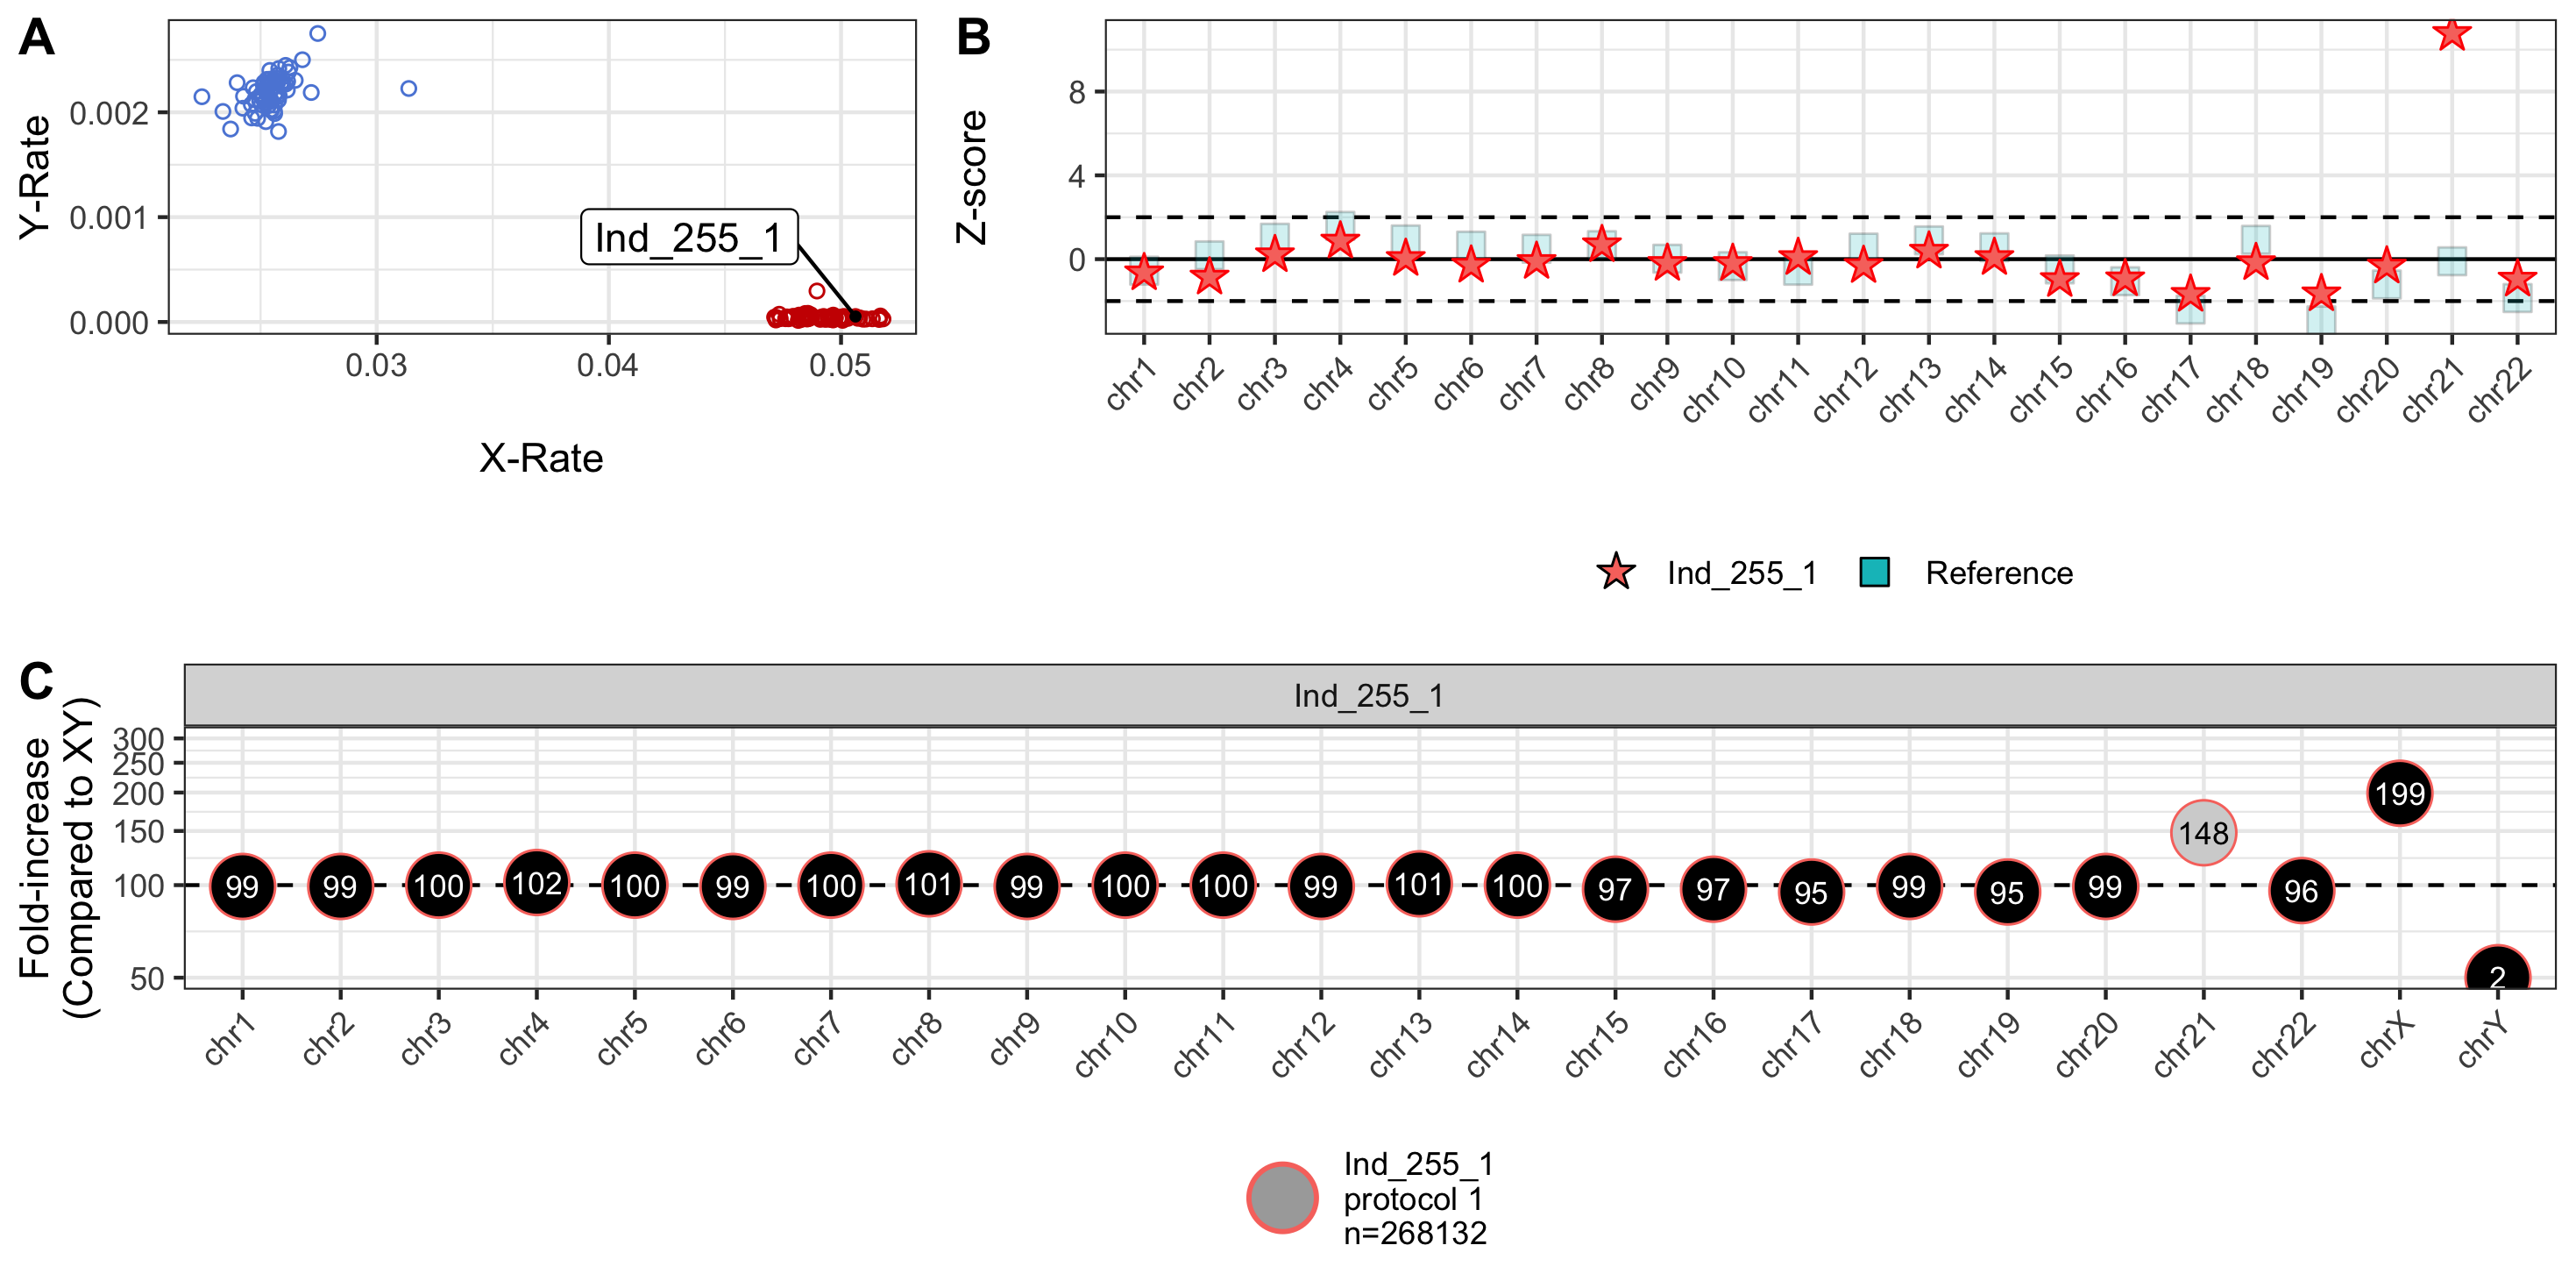
\includegraphics[keepaspectratio]{figs/trisomy21Diagnostic.png}}

}

\caption{The three-panel diagnostic plot for individual Ind\_255\_1
confirming the assignment of XX and trisomy
21.\label{fig:diagnosticT21}}

\end{figure}%

\section{\texorpdfstring{Conclusion\label{sec:end}}{Conclusion}}\label{conclusion}

This article describes the usage and functionality of the R package
\texttt{RChASM}. This package is used to assign autosomal and sex
chromosomal aneuploidies, even in cases where only 60,000 mapped reads
were recovered, which is equivalent to coverage as low as 0.001X
(assuming a mean read length of approximately 45 bp). \texttt{RChASM}
returns posterior probabilities for each of the possible karyotypes, and
because XX and XY are in the set of possible sex chromosomal karyotypes,
can be used for genetic sex assignment. Additionally, \texttt{RChASM}
returns goodness of fit statistics per individual to assess (a) if the
observed read counts are consistent with the reference distribution, (b)
which chromosomes are over- or under-represented by the number of mapped
reads compared to expectation, and (c) whether contamination between an
XX and XY individual may explain the assignment of XXY better than a
true XXY karyotype.

\texttt{RChASM} is limited by the fact that it requires reference data
containing at least 30 observations, but in fitting a
Dirichlet-multinomial model for each unique analysis, can be applied to
any type of sequencing data. However, to best help alleviate this
limitation, we also include with \texttt{RChASM} a reference data set of
globally produced shotgun-derived and 1240k-derived read counts.

We encourage researchers to consider this limitation when using
\texttt{RChASM}. However, as all methods have different strengths and
weaknesses, we encourage researchers to use multiple methods for
detecting chromosomal aneuploidies, such as Karyo\(R_{x}R_{y}\). For
further ease of use in pre-processing bam files into read counts, we
also include a script that employs widely-used standard software
(samtools, bedtools, R, bash, perl).

\section{Data description}\label{data-description}

A full explanation of the data used in this analysis can be found in the
publication of the ChASM methodology (Rohrlach et al. 2026).

\section{Author contributions}\label{author-contributions}

Adam B. Rohrlach conceived, designed and implemented the method, wrote
the paper, prepared the figures, performed the computation work,
reviewed drafts of the paper and edited submissions.

Jonathan Tuke submitted the package to CRAN, reviewed drafts of the
paper and edited submissions.

Kay Prüfer created and implemented the software for pre-processing bam
files, reviewed drafts of the paper and edited submissions.

Wolfgang Haak wrote the paper, reviewed drafts of the paper and edited
submissions.

\section{Acknowledgements}\label{acknowledgements}

We thank Associate Professor Elina Salmela, Nigel Bean and Vincent
Braunack-Mayer for important and enlightening discussions regarding the
manuscript, and Johannes Krause and the Max Planck Society for the
support in producing this software.

\section{Funding}\label{funding}

This research was financed by the Max Planck Society and the European
Research Council under the European Union's Horizon 2020 research and
innovation programme (grant agreement number 101141408-ROAMANCE, W.H.).

\section*{Bibliography}\label{bibliography}
\addcontentsline{toc}{section}{Bibliography}

\protect\phantomsection\label{refs}
\begin{CSLReferences}{1}{1}
\bibitem[\citeproctext]{ref-anastasiadou2024detection}
{Anastasiadou, Kyriaki, Marina Silva, Thomas Booth, et al.} 2024.
{``Detection of Chromosomal Aneuploidy in Ancient Genomes.''}
\emph{Communications Biology} 7 (1): 14.

\bibitem[\citeproctext]{ref-hassold2001err}
Hassold, Terry, and Patricia Hunt. 2001. {``To Err (Meiotically) Is
Human: The Genesis of Human Aneuploidy.''} \emph{Nature Reviews
Genetics} 2 (4): 280--91.

\bibitem[\citeproctext]{ref-mathieson2018genomic}
{Mathieson, Iain, Songül Alpaslan-Roodenberg, Cosimo Posth, et al.}
2018. {``The Genomic History of Southeastern {Europe}.''} \emph{Nature}
555 (7695): 197--203.

\bibitem[\citeproctext]{ref-nagaoka2012human}
Nagaoka, So I, Terry J Hassold, and Patricia A Hunt. 2012. {``Human
Aneuploidy: Mechanisms and New Insights into an Age-Old Problem.''}
\emph{Nature Reviews Genetics} 13 (7): 493--504.

\bibitem[\citeproctext]{ref-orr2015aneuploidy}
Orr, Bernardo, Kristina M Godek, and Duane Compton. 2015.
{``Aneuploidy.''} \emph{Current Biology} 25 (13): R538--42.

\bibitem[\citeproctext]{ref-rohrlach2026chasm}
Rohrlach, Adam B, Jonathan Tuke, Kay Prüfer, and Wolfgang Haak. 2026.
{``{ChASM}: A Statistically Rigorous Method for the Detection of
Chromosomal Aneuploidies in Ancient {DNA} Studies.''}
\emph{Bioinformatics} 42 (5): btag204.

\bibitem[\citeproctext]{ref-samango2013snp}
{Samango-Sprouse, Carole, Milena Banjevic, Allison Ryan, et al.} 2013.
{``{SNP}-Based Non-Invasive Prenatal Testing Detects Sex Chromosome
Aneuploidies with High Accuracy.''} \emph{Prenatal Diagnosis} 33 (7):
643--49.

\bibitem[\citeproctext]{ref-skuse2018sex}
Skuse, David, Frida Printzlau, and Jeanne Wolstencroft. 2018. {``Sex
Chromosome Aneuploidies.''} \emph{Handbook of Clinical Neurology} 147:
355--76.

\bibitem[\citeproctext]{ref-venter2001sequence}
{Venter, J Craig, Mark D Adams, Eugene W Myers, et al.} 2001. {``The
Sequence of the Human Genome.''} \emph{Science} 291 (5507): 1304--51.

\end{CSLReferences}




\end{document}
